\chapter{Implementation}

This chapter provides an overview of the important implementation details about the HaptiQ, as described in the Design chapter. 
Firstly, the hardware implementation is discussed, followed by the API. A dedicated section will discuss the tactons implementation. Finally, implementation details about the two example applications are covered in the last section of this chapter.

\section{The Hardware}

Building the hardware components of the two HaptiQ devices has been a challenge on its own. Both the 4-HaptiQ and the 8-HaptiQ are 3D-modelled using Google Sketchup \footnote{Google SketchUp. \url{http://www.sketchup.com} . [Online; last checked: 03/04/2014].}. Models are then exported in the STL format, a standard in CAD software, and commissioned to a 3D printer. I used a MakerBot\textregistered   Replicator\texttrademark 2x. This is an experimental 3D printer, therefore high precision (\textless 2mm) is hard to achieve and requires many attempts before being able to print the wanted model. 

Phidgets boards\footnote{Phidges. \url{http://www.phidgets.com/} . [Online; last checked: 04/04/2014].} are used to control the micro servomotors, \textit{Hitech HS-65MG}\footnote{HITECH RCD USA. \url{http://hitecrcd.com/} . [Online; last checked: 04/04/2014].}, and get pressure inputs, via force-sensing resistors. The wiring is more of a demanding task, rather than a challenging one, requiring many hours of work.

The different components of the device are assembled using super glue and screws (see the HaptiQ manual for more information on printing and assembling the device). 

\subsection{Fiducial Markers}

The provided API supports the recognition of two types of fiducial markers: Microsoft Bytetags and GRATF glyphs. The HaptiQs, built for this project, place the fiducial markers on the bottom side. However, in the case of the the GRATF glyphs, the fiducial marker can also be placed on top of the device. This is true if we assume that an appropriate structure around the HaptiQ is built, and a web-cam or similar is used to retrieve top-view images of the device with the glyph.

\begin{figure}
        \centering
        \begin{subfigure}[H]{0.3\textwidth}
                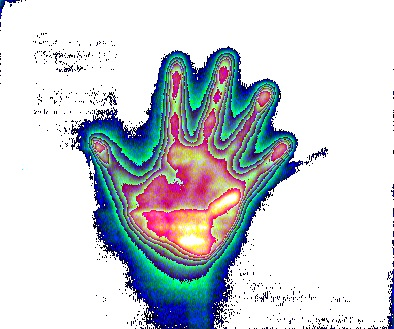
\includegraphics[width=\textwidth,height=\textwidth]{hand.jpg}
                \caption{Raw image of Hand}
                \label{fig:rawHand}
        \end{subfigure}%
        ~ %add desired spacing between images, e. g. ~, \quad, \qquad etc.
          %(or a blank line to force the subfigure onto a new line)
        \begin{subfigure}[H]{0.3\textwidth}
                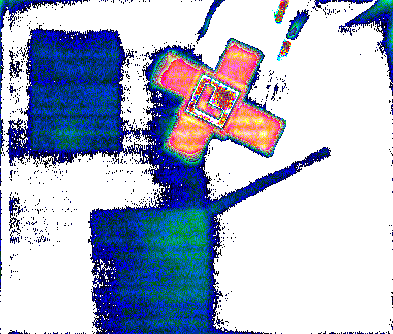
\includegraphics[width=\textwidth,height=\textwidth]{type1.png}
                \caption{Raw image of 4-HaptiQ with Glyph - type 1}
                \label{fig:rawHaptiQ1}
        \end{subfigure}
        ~ %add desired spacing between images, e. g. ~, \quad, \qquad etc.
          %(or a blank line to force the subfigure onto a new line)
        \begin{subfigure}[H]{0.3\textwidth}
                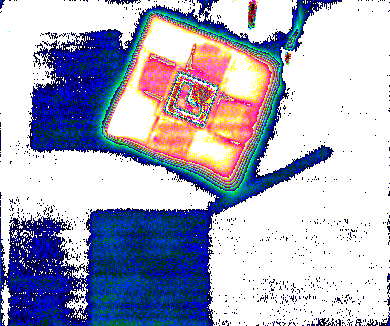
\includegraphics[width=\textwidth,height=\textwidth]{type2.png}
                \caption{Raw image of 4-HaptiQ with Glyph - type 2}
                \label{fig:rawHaptiQ2}
        \end{subfigure}
        \caption{Raw images}\label{fig:rawImages}
\end{figure}

The Bytetags, according to Microsoft, can be printed on standard office paper \footnote{MSDN. Printing Tagged Objects. \url{http://www.msdn.microsoft.com/en-us/library/ee804862(v=surface.10).aspx/}. [Online; last checked: 04/04/2014].}. However, during the first iteration phase of this project it was evident that printed Bytetags lead to poor results, with the fiducial markers being tracked at low frequency.

The alternative solution is to use glyphs. The Surface SDK 2.0 allows to retrieve raw image data from the interactive table. Having access to this data, it is possible to apply classical image matching algorithms to identify particular objects. This is achieved using GRATF, a C\# library that allows recognition and localization of glyphs in still images. 

Figure ~\ref{fig:rawImages} shows three raw images retrieved through the Surface SDK 2.0. The Microsoft PixelSense uses near-infrared sensors. Figure ~\ref{fig:rawHand}, for instance, represents how the hand absorbs infrared light, rather than its heat values as one may think. Glyphs are $n \times n$ grids, with n from 5 to 8, where each cell is either black or white (see Figure  ~\ref{fig:glyph}) and minimum side length of 8mm, that can be printed using Glyph Recognition Studio \footnote{Glyph Recognition Studio. Available at \url{http://www.aforgenet.com/projects/gratf/}. [Online; last checked: 04/04/2014].}. Additional rules apply, such that that the border cells can only be white and the glyph cannot be symmetrical in any of its axis. The base of the HaptiQ is covered with white paper, so that the black tiles in the glyphs are recognised more easily (see Figure ~\ref{fig:rawHaptiQ1}). However, this is not sufficient for the glyph to be recognised at all angles. After testing glyphs of different dimensions and on different surfaces, I found out that extending the glyph with low absorption material (e.g. white foam board) improves the recognition of the glyph significantly (see Figures ~\ref{fig:rawHaptiQ2} and ~\ref{fig:whitesurface}).   

\begin{figure}[H]
  \centering
  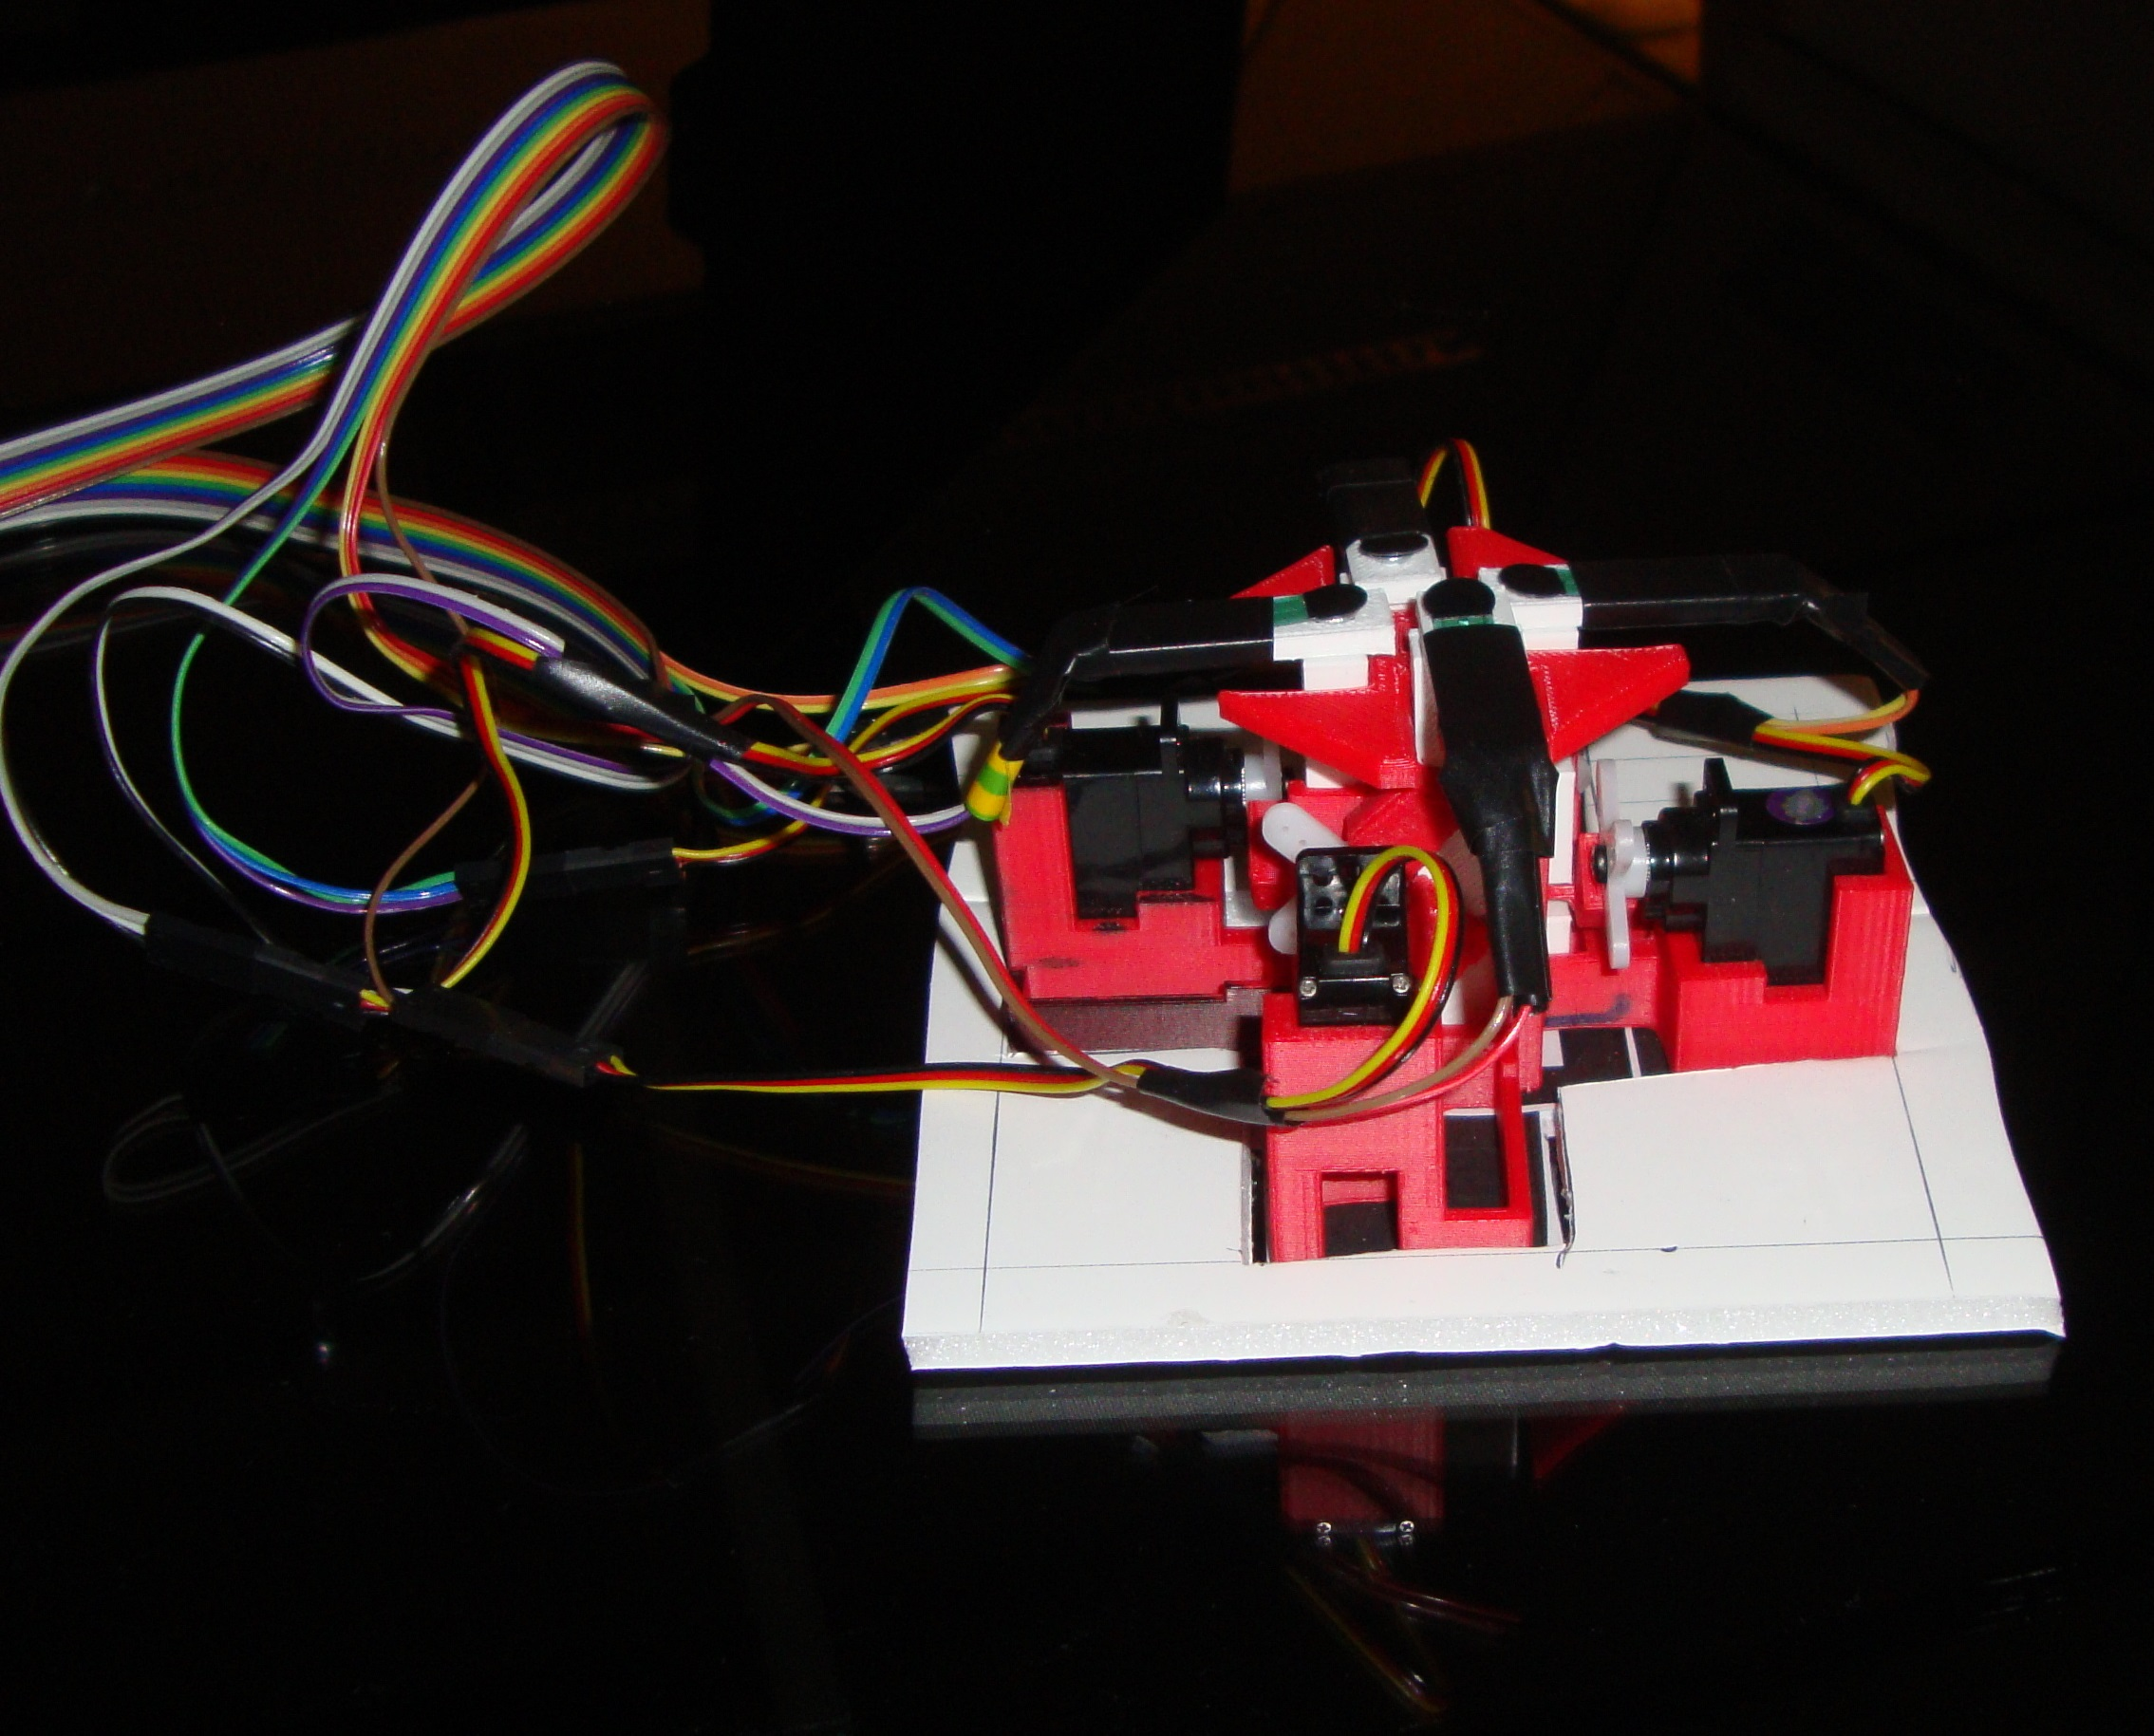
\includegraphics[width=0.5\textwidth]{DSC06783.JPG}
  \caption{HaptiQ with extended white board base}
  \label{fig:whitesurface}
\end{figure}

\section{The API}

\subsection{Input API}

The Input API is the component used to retrieve the HaptiQ location on the tabletop. It follows that this is highly hardware dependent on the used hardware, especially on the type of interactive surface. The current targeted hardware comprehends the Microsoft Tabletops using the Surface SDK 2.0. Code to retrieve image data from web-cams is also provided. 
As explained in the design section, two main classes exist in the Input API: one to recognise Bytetags and one to recognise glyphs.

Recognising the Bytetags is straightforward. This is done through the \textit{TouchTarget} object of the \textit{Microsoft.Surface.Core} library. On the other hand, glyphs are recognised by calling the \textit{FindGlyphs} function, from the GRATF library, on a bitmap image. GRATF does not provide any functionality to estimate the position and the rotation of the glyphs. However, when a glyph is recognised, all its vertices are known. The position is estimated by calculating the crossing point between the two diagonals of the glyph. The rotation, instead, is estimated using the inclination angle of one of the edges of the glyph. 

The API raises events of the form:
\lstset{style=sharpc1}
\begin{lstlisting}
delegate void ChangedEventHandler(object sender, InputIdentifier inputIdentifier, Point point, double orientation, EventArgs e);
\end{lstlisting}

in order to notify the current location of a device, recognisable by a unique identifier (Bytetag or glyph). Then the HaptiQsManager, from within the HaptiQ API, handles such events.  

It is important to note that Bytetags are supported for debugging purposes only. Working with the provided tabletop is time consuming. Allowing Bytetags to be used, it is possible to run, debug and test the system using the Input Simulator provided with the Surface SDK 2.0 using a normal machine. 

\subsection{HaptiQ API}

The HaptiQ API, as previously stated, controls the device and coordinates its work with the other two main components: the Input API and the applications. The \textit{HaptiQsManager}, the \textit{HaptiQ}, and the \textit{Actuator} classes play the major role in controlling the devices and ensuring the coordination between input locations, haptic objects and behaviours. These three classes are also dependent on the Phidget library \footnote{Phidgets. Library available at \url{http://www.phidgets.com/}. [Online; last checked: 04/04/2014].}. 

On the creation of the manager, the configuration process is launched (see section ~\ref{sec:configuration} for more details about devices configuration) and HaptiQ instances are created appropriately. The manager assigns each device a unique ID, which can be used to find and access a device. 
Each HaptiQ keeps track of its own actuators, the connected pressure sensors, and the current behaviours to play. After an HaptiQ instance is initialised in the constructor, an independent thread is initiated. This consists of a loop that runs all the current behaviours every 10ms. Reducing the frequency gradually decreases the smoothness of the played dynamic behaviours. On the other hand, increasing the frequency creates an unnecessary overuse of resources. 

A behaviour consists of a dictionary mapping an actuator of the device to its wanted position. The position is expressed as a value between 0 and 1, where 0 indicates that the actuator should be moved to its minimum position, and 1 to its maximum position. The manager retrieves behaviours to be played, from each haptic object, and distributes them to the devices that generated them. Nonetheless, an HaptiQ instance allows behaviours to be explicitly added or removed, giving more flexibility to clients. Similarly to the HTP toolkit, behaviours can be combined by averaging the positions for each actuator. 
Actuators are independent from each other, therefore it is possible to exploit parallelism using a parallel for-loop as shown in Code ~\ref{lst:parallelActuators}.

The Actuator class wraps an \textit{AdvancedServoServo} from the Phidget library, used to control a single servo motor, and keeps track of the current pressure applied by the user. 

\lstset{style=sharpc1}
\begin{lstlisting}[caption={Parallelising Actuators},label={lst:parallelActuators}]
Parallel.ForEach(actuators, entry => 
                    {
                        this.setActuatorPositionByPercentage(entry.Key, entry.NormalisedPosition);
                    });
\end{lstlisting}

\subsubsection{Pressure Events}

The HaptiQ class defines two types of pressure events: pressure changes and pressure gestures. The first type of event is raised whenever the pressure registered by a sensor changes. The second type instead is raised on pressure gestures being recognised. The current API supports only one type of gesture: a \textit{press}. A press is recognised whenever the pressure registered by a particular sensor increases over a certain threshold and then rapidly decreases within a certain time frame (see Figure ~\ref{fig:pressureValues}). 

Time-series analysis could allow the recognition of other gestures, but this is outside the scope of the project.


\begin{figure}[H]
  \centering
  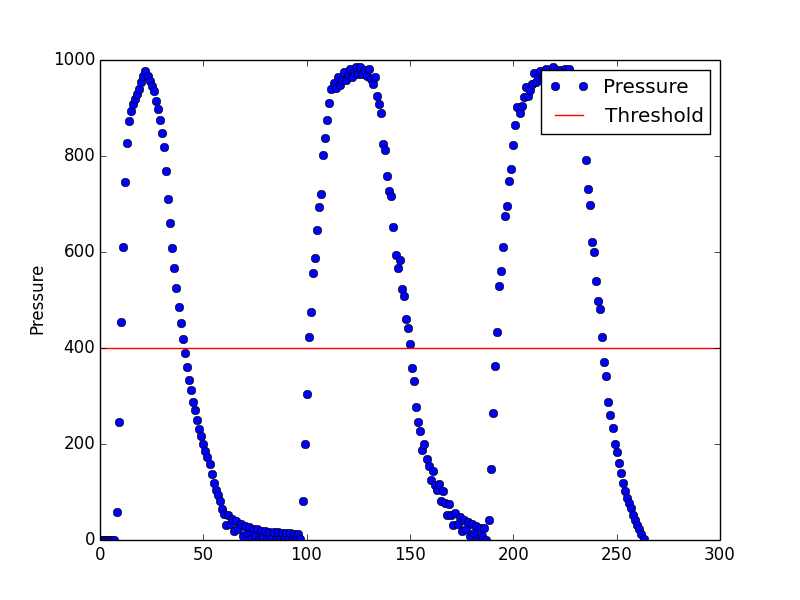
\includegraphics[width=0.7\textwidth]{pressureValues.png}
  \caption{Three consecutive press gestures. Note that x-axis does not represent time.}
  \label{fig:pressureValues}
\end{figure}

\subsubsection{Haptic Objects}

Haptic objects are visual elements that client applications can use to represent information to the visually impaired. An Haptic object must implement the IHapticObject interface. This interface, as shown in Code ~\ref{lst:IHapticObject}, consists of three main methods:

\begin{itemize}
	\item \textbf{handleInput}: called whenever a new input location is received from the Input API. This method returns a Tuple of three elements: a rule to apply for the returned values (\textit{ADD}, \textit{REMOVE}, \textit{SUBSTITUTE}, \textit{NONE}) and two behaviours. For instance, the method may add a new behaviour to the HaptiQ, or substitute the current behaviour with a new one. Since HaptiQs can combine behaviours, each HaptiQ object needs to keep track of what current behaviour is assigned to each HaptiQ. 
    \item \textbf{handlePress}: called when a pressure gesture event is raised
    \item \textbf{registerAction}: allows clients to register custom actions to be executed on \textit{handlePress}. For example, a \textit{BasicAction} allows the client to specify text to be read out through the speakers when a pressure gesture is fired.
\end{itemize}

\lstset{style=sharpc1}
\begin{lstlisting}[caption={IHapticObject},label={lst:IHapticObject}]
public interface IHapticObject 
{
  Tuple<BEHAVIOUR_RULES, IBehaviour, IBehaviour> handleInput(HaptiQ haptiQ);
  
  void handlePress(HaptiQ haptiQ);
  
  void registerAction(IAction action);
}
\end{lstlisting}

The API provides the \textit{HapticShape} abstract class, which implements \textit{IHapticObject} and extends \textit{Shape}, from the WPF Windows Shapes. Clients, therefore, have access to haptic objects usable on WPF applications, but can also create their own custom shapes, by implementing \textit{IHapticObject}, for XNA applications. 

The \textit{HapticShape} class provides the implementation of \textit{handleInput} and provides other useful functions, such as the possibility to add textual information to a shape. The implemented \textit{handleInput} method ensures that states (\textit{UP} or \textit{DOWN}) and behaviours of a current HaptiQ, for a specific shape, are updated correctly. Classes extending \textit{HapticShape}, such as \textit{HapticRectangle} or \textit{HapticCircle}, need to implement the method

\lstset{style=sharpc1}
\begin{lstlisting}
IBehaviour chooseBehaviour(HaptiQ haptiQ);
\end{lstlisting}

which returns the behaviour that should be played by the given device, at a particular state (see Section ~\ref{sec:designTactons} for the tactons used by the provided shapes).

Finally, objects extending \textit{HapticShape} are renderable on WPF applications. These are rendered only when the object is added to a canvas or grid within the client application.

\section{Configuration}
\label{sec:configuration}

The two prototypes created in this project have different characteristics. For instance, the second version has eight actuators, rather than four, and its servos have a certain action range that the first version does not have. The API allows devices with different characteristics to be used by serializing their configurations as XML files. On creation, the manager inspects the current directory for XML configuration files\footnote{Pattern used to name configuration files is: 'CONFIG\_*.xml'} and attempts to create HaptiQs using the deserialized configurations and the attached Phidget boards.  

But even so, it could be the case that no configuration file exists for an attached HaptiQ. This is especially true the first time a device is used. In this eventuality a configuration form is prompted to the user (see Figure \ref{fig:configurationPanel}). The form has been created using \textit{WinForms}, so that no dependency on WPF or similar library is added. The panel allows users to specify which actuators to use, their range of action, whether to use pressure input or not, and the fiducial marker to use. 

Users are prompted with a configuration form until all attached Phidget boards are configured.

\begin{figure}[H]
  \centering
  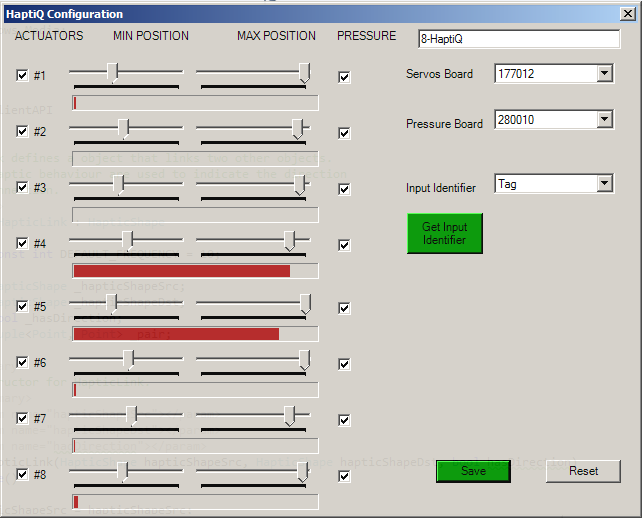
\includegraphics[width=0.7\textwidth]{configuration.png}
  \caption{Configuration Form}
  \label{fig:configurationPanel}
\end{figure}

\section{Tactons}

Tactons, or behaviours, represent the way the actuators of the HaptiQ move to represent shapes, edges, and directions. This section gives an overview of the behaviours implementation.

Each behaviour must implement the play method:

\lstset{style=sharpc1}
\begin{lstlisting}
abstract Dictionary<int, double> play();
\end{lstlisting}

which returns a dictionary mapping actuators to their desired positions. 
This is the only requirements that has to be satisfied whenever a new behaviour is created. In addition, tactons can be dynamic. Therefore, the \textit{Behaviour} abstract class provides an internal timer that behaviours should update at each call to \textit{play}. 

Being able to map an HaptiQ to basic behaviours, such as \textit{Flat} and \textit{Max}, is fairly simple because there is no dependence on previous states of the behaviour or the position and orientation of the device relative to a segment (e.g. Pulsation behaviour). The initial approach consisted in hard-coding all possible cases as shown in Code ~\ref{lst:tactonsInitialApproach}. This example is valid only for the 4-HaptiQ. It becomes clear that as the number of actuators increases, the code will also increases in size and eventually becomes unmaintainable. 

\lstset{style=sharpc1}
\begin{lstlisting}[caption={Tactons - Initial approach},label={lst:tactonsInitialApproach}]
private int[][][] directionMatrix = new int[][][]
                    {  new int[][]{                 // vertical 
                        new int[]{0, 1, 0, 1, 0}, 
                        new int[]{1, 1, 1, 0, 0}, 
                        new int[]{0, 0, 1, 0, 1}, 
                        new int[]{1, 1, 0, 0, 1}, 
                        new int[]{0, 1, 0, 1, 0}, 
                        new int[]{1, 1, 1, 0, 0}, 
                        new int[]{0, 0, 1, 0, 1}, 
                        new int[]{1, 1, 0, 0, 1}}, 
                    new int[][]{                    // horizontal
                        new int[]{0, 0, 1, 0, 1},
                        new int[]{1, 1, 0, 0, 1},
                        new int[]{0, 1, 0, 1, 0},
                        new int[]{1, 1, 1, 0, 0},
                        new int[]{0, 0, 1, 0, 1},
                        new int[]{1, 1, 0, 0, 1},
                        new int[]{0, 1, 0, 1, 0},
                        new int[]{1, 1, 1, 0, 0}},
                   ...
                   };
\end{lstlisting}

The second approach generalises the initial approach, by representing actuators as bits, rather than integers within arrays, and applying bitwise operations (see Figure ~\ref{fig:bits}). 

For example, to represent a vertical line in the 4-HaptiQ, we can just use the number five:

		0101 (5) = 0001 (1) \& 0100 (4) \\
Shifting numbers to right (or left) with carry allows behaviours to choose what actuators to use. 
The shifting offset is based on the orientation of the device compared to the segment it has to represent. Finding this value consists into subdividing the HaptiQ in logical sectors. For instance, the 4-HaptiQ is divided in eight sectors (see Figure ~\ref{fig:sectors}). Even sectors, in red, represent states that the device needs to represent by alternating actuators over time.

Say that 0101 is valid for the first sector, then when the device is in the third sector a shift by one only is needed: $0101 \gg 1$ = 1010 (with carry). For the case of even sectors, bits are not ended, but applied conditionally on the internal timer value:

		0001 (timer mod 2 == 0)
        
        0100 (timer mod 2 != 0)

\begin{figure}[H]
  \centering
  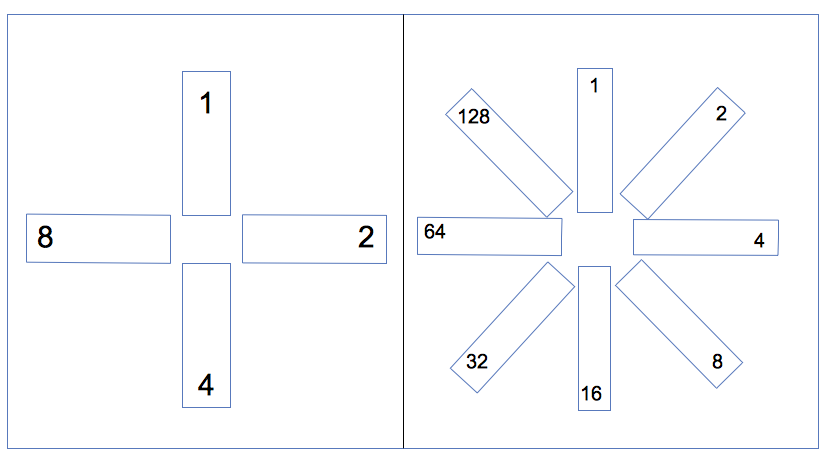
\includegraphics[width=0.7\textwidth]{bits.png}
  \caption{Actuators bits representation}
  \label{fig:bits}
\end{figure}

\begin{figure}[H]
  \centering
  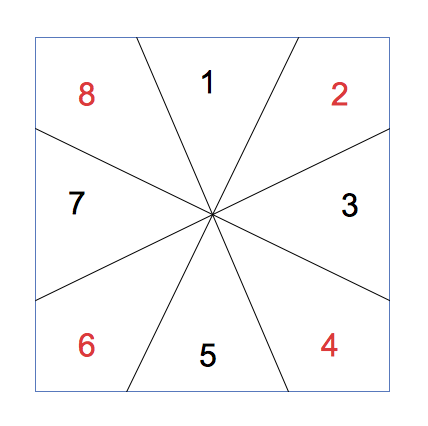
\includegraphics[width=0.4\textwidth]{sectors.png}
  \caption{4-HaptiQ sectors}
  \label{fig:sectors}
\end{figure}

Similar bitwise operations, as described above, are applied for the direction, pulsation, and linear tactons. The notification tacton, however, takes a different approach since each actuator can be in different states (see Section \ref{sec:notification}). The solution used is to use a 2-D array with values $[position, direction]$ for each actuator, where the direction indicates whether the position should increase or decrease in the current iteration. The direction is inverted when the minimum or maximum allowed position is reached.  

\section{A basic example}

In this section, I will show how to use the API using a simple example (see Code ~\ref{lst:basicAPIUsage}). This section is necessary to properly understand section ~\ref{sec:Applications}, which discusses the provided example applications of this project.

The first step consists in creating a WPF application and adding a reference to the HaptiQ\_API. In the design view, add a Grid named \textit{container} to the main window. Import the HaptiQ\_API in the code view of the application. 

The call \textit{HaptiQsManager.Create(windowTitle, \textless Input Class\textgreater)} initialises the HaptiQ device and the Input API, using the specified Input class (e.g. 'SurfaceInput' for Bytetags). 
Objects are automatically added to the system when they are created. These are rendered only when added to a WPF grid or canvas. 

In the \textit{OnClosed} method of the WPF application, it is important to call \textit{HaptiQsManager.Instance.delete()} to ensure that the HaptiQs are detached correctly and all resources are disposed correctly.

\lstset{style=sharpc}
\begin{lstlisting}[caption={Basic API usage},label={lst:basicAPIUsage}]
using HaptiQ_API;

public partial class Application : SurfaceWindow
{
  public Application()
  {
      HaptiQsManager.Create(windowTitle, ''SurfaceInput'');
      
      HapticShape rect0 = new HapticRectangle(50, 50, 150, 200);
      rect0.color(Brushes.Salmon);
      this.container.Children.Add(rect0);
      
      HapticShape rect1 = new HapticRectangle(150, 350, 200, 200);
      rect1.color(Brushes.Orange);
      this.container.Children.Add(rect1);
      
      HapticShape rect2 = new HapticRectangle(550, 150, 100, 100);
      rect2.color(Brushes.Green);
      this.container.Children.Add(rect2);
      
      HapticShape link = new HapticLink(rect2, rect1, true);
      link.color(Brushes.White);
      this.container.Children.Add(link);
  }
  
  protected override void OnClosed(EventArgs e)
  {
      base.OnClosed(e);
      HaptiQsManager.Instance.delete();
      Application.Current.Shutdown();
  }
}
\end{lstlisting}

\begin{figure}[H]
  \centering
  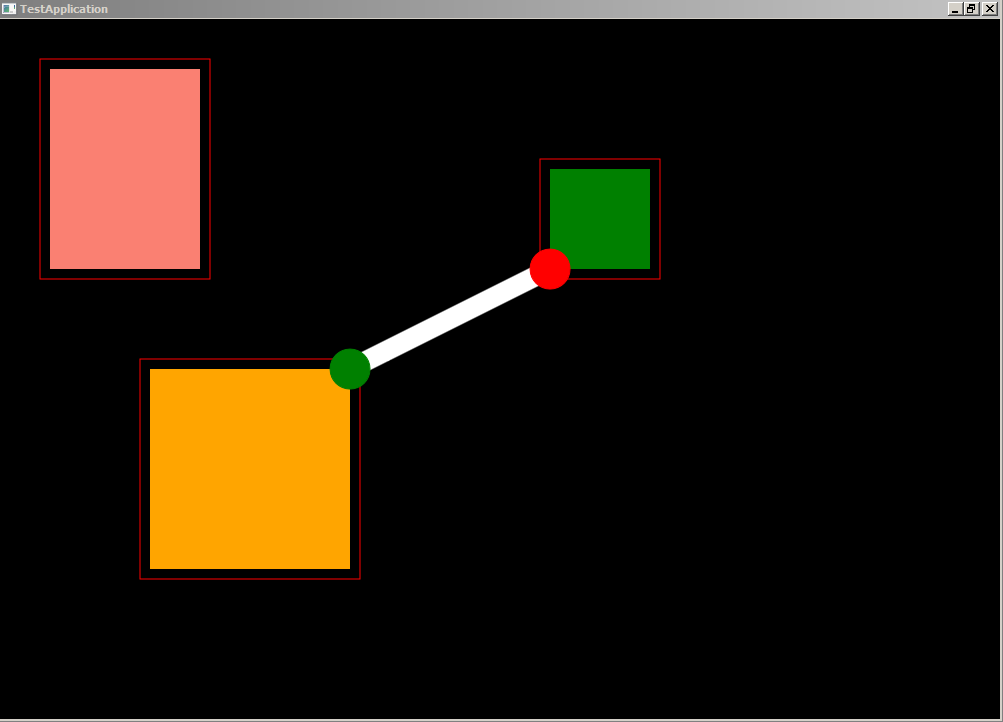
\includegraphics[width=0.5\textwidth]{basic_example.png}
  \caption{Basic API usage}
  \label{fig:basicexample}
\end{figure}

Please refer to the HaptiQ manual for further details and additional examples on how to use the API. 


\section{Applications}
\label{sec:Applications}

This section will briefly explain some of the implementation details about the two example applications provided with this project. 

\subsection{Graph Visualiser}

The graph visualiser application, as explained in section ~\ref{sec:graphVis}, provides basic functionality to build and visualise graphs that can be perceived using the HaptiQ. 
The main user interface is created using Visual Studio to organize the WPF standard controls (i.e. buttons). A click handler is attached to each button. Two types of buttons exist in the application. The first type are used to create new haptic objects, while the second one to make the objects selectable or not. \\
When the first type of buttons is used, a new window is shown allowing the user to choose the properties of the haptic object. A create button in the new window adds the haptic object to the main window, as shown in Code ~\ref{lst:basicAPIUsage}.
The second type, instead, iterates over all the haptic objects through the \textit{HaptiQsManager} and make them selectable or not. This functionality is useful because we want objects to be selectable only when creating the graph and not when the user is sensing it.  


\subsection{Function Visualiser}

The function visualiser application is self-contained in one simple C\# class. A user can input basic functions (e.g. linear, trigonometric) via the interface provided by the application. The interface, similarly to the Graph Visualiser one, is created with the assistance of Visual Studio. \\
The application accepts only functions of the form: $ y = f(x) $, with only one occurrence of x. Functions are evaluated using the NCalc library \footnote{NCalc. Library Available at \url{http://www.ncalc.codeplex.com/}. [Online; last checked: 02/04/2014].} at regular intervals over x. The pseudocode ~\ref{lst:functVisPseudo} shows the use of the NCalc library and the creation of the HapticPolyline. 

\lstset{style=sharpc1}
\begin{lstlisting}[caption={Function Visualiser pseudocode},label={lst:functVisPseudo}]
var regex = new Regex(Regex.Escape("x"));
for(int i = 0; i < RANGE; i++)
{
  var function = regex.Replace(inputTextFunction, i.ToString(), 1);
  NCalc.Expression expr = new NCalc.Expression(function);
  var y = expr.Evaluate();
  points.add(new Point(i, y));
}

HapticShape polyline = new HapticPolyline(points);
polyline.color(Brushes.White);
container.Children.Add(polyline);

\end{lstlisting}